\chapter{Related Work}

In this section we discuss the methods for computing indirect illumination relevant to our thesis. Although radiosity and photon mapping are other popular global illumination algorithms, we did not have freely available implementations that would accept our scene format, and in the interest of scope, we did not implement our own versions. We do not cover them here and leave it to the reader if further knowledge of the subject area is desired \cite{bib:radiosity, bib:photon_maps}.

We first cover the Monte Carlo gather method, which we have implemented for comparison with our GPU PBCB algorithm. This method produces highly realistic results, but at the cost of copious computation, which in our experience, can easily require multiple hours of rendering time on commodity hardware. Our GPU PBCB algorithm is meant to produce comparable results, much faster.

We also discuss the basic PBCB algorithm, which we have extended to leverage the rasterization power of the GPU. The PBCB algorithm as developed by Christensen at Pixar \cite{bib:christensen2008} utilizes a software-based rasterization. It is here that we feel leveraging the power of the GPU can accelerate the algorithm and produce faster render times.

Lastly, a promising area of research that we do not cover here is maximal Poisson disk point set generation on 3D surfaces \cite{bib:poisson_set}. The goal of this research is similar to our surfel generation goal; that is to say, they both strive for uniform distribution of points on 3D surfaces. Although the technique presented in \cite{bib:poisson_set} does not address transformed spheres or boxes, it may be possible to extend their ideas to cover these types of geometry.

%-------------------------------------------------------------------------------
% SECTION: Monte Carlo Gather
%-------------------------------------------------------------------------------
\section{Monte Carlo Gather}
\label{sec:monte_carlo_gather}

\begin{figure}
    \centering
    \subfloat{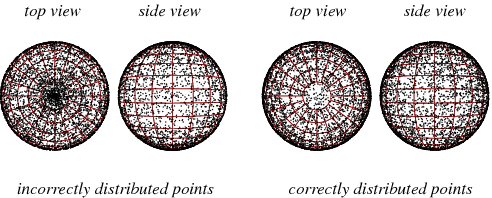
\includegraphics[width=150mm]{../img/SphericalDistribution.png}}
    \caption[Sphere Point Distribution]{Point distribution on a sphere: left is na\"{\i}ve point sampling that results in higher point density near the poles, right is correct sampling \cite{bib:point_sampling_wa}.}
    \label{fig:sphere_sampling}
\end{figure}

The Monte Carlo gather method is used in ray-tracing for indirect illumination, and receives its name from the Monte Carlo integration approximation discussed in Section \ref{sec:monte_carlo_integration}. Instead of computing the true outgoing radiance integral, which is all but impossible except in the simplest of cases, we discretize the integral and compute its approximation. We begin our description of this method at the time a ray-geometry intersection is found.

The first step is to generate the randomized sample vectors used to discretize the integral over the hemisphere. To this end, the algorithm leverages a hemisphere sampler: a function that takes two floating point variables as input, and produces a sample point on the hemisphere, see Figure \ref{fig:sphere_sampling} (it should be noted that identical input always results in identical output). Typically, samplers are designed to produce a uniform random distribution over the hemisphere when two uniform random variables, $u_{1}$ and $u_{2}$, are used as input. The following equations \cite{bib:pbr} describe this mathematically:
\begin{eqnarray}
x &=& \cos (2 \pi u_{2}) \sqrt{1-u_{1}^{2}} \nonumber \\
y &=& \sin (2 \pi u_{2}) \sqrt{1-u_{1}^{2}} \nonumber \\
z &=& u_{1}
\label{eqn:uniform_hemisphere}
\end{eqnarray}

However, in some cases a uniform distribution over the hemisphere is not desired. We have found that using a purely uniform random distribution over the hemisphere does not result in visually acceptable noise levels until we reach approximately 256 sample vectors (see Figure \ref{fig:monte_carlo_noise}).

In the case of indirect illumination computation, sample points near the top are more highly weighted then those near the bottom due to the $n \cdot l$ factor used in the Phong Shading model (see Section \ref{sec:phong_model}). Therefore, a technique called importance sampling \cite{bib:pbr} is used to create a non-uniform sampling (even though the input variables are from a uniform distribution) of the hemisphere, where the sample density increases where the $n \cdot l$ factor is largest: the top of the hemisphere. We refer to this as a cosine-weighted hemisphere sampler because the likelihood of generating a given sample point is proportional to the cosine of the angle between the vector represented by the sample point and the unit hemisphere's vertical vector \textless$0,1,0$\textgreater. This is described mathematically in equation \ref{eqn:cosine_hemisphere} \cite{bib:pbr}.
\begin{eqnarray}
x &=& \cos (2 \pi u_{2}) \sqrt{u_{1}} \nonumber \\
y &=& \sin (2 \pi u_{2}) \sqrt{u_{1}} \nonumber \\
z &=& \sqrt{1-x^{2}-y^{2}}
\label{eqn:cosine_hemisphere}
\end{eqnarray}

An algorithm implementing equation \ref{eqn:cosine_hemisphere} is used to generate a desired number of cosine-weighted sample points on a unit hemisphere. These sample points are treated as vectors to describe the direction of sample rays used to gather incoming radiance information. In order to convert from a vector in unit hemisphere coordinates to a vector in world space coordinates we use Algorithm \ref{alg:unit_world_xform}. This is a standard coordinate system transformation between surface, or object, space and world space.

\begin{algorithm}[H]
\captionfont
\caption[Unit to World Hemisphere]{Transform from unit hemisphere to world space.}
\label{alg:unit_world_xform}
{\fontsize{10}{9}\selectfont
\begin{algorithmic}
   \Function{HemisphereTransform}{$surfaceNormal$}
      \If{$|surfaceNormal.y| = 1$}
         \State $tangent$ :=  $\textless1,0,0\textgreater$
      \Else
         \State $k := \textless0,1,0\textgreater$
         \State $tangent$ :=  $k - ((k \cdot surfaceNormal)*surfaceNormal)$ //Gram-Schmidt Process
         \State normalize($tangent$)
      \EndIf
      \State $binormal := surfaceNormal \times tangent$
      \State $transform := \bigl( \begin{smallmatrix} tangent.x & surfaceNormal.x & binormal.x \\ tangent.y & surfaceNormal.y & binormal.y \\ tangent.z & surfaceNormal.z & binormal.z \end{smallmatrix} \bigr)$
      \State \Return $transform$
   \EndFunction
\end{algorithmic}
}
\end{algorithm}

The next step is to use these transformed vectors as ray directions to perform a recursive ray tracing computation. Each computation returns the incoming radiance, just as the primary rays return incoming radiance written to a final image pixel. These incoming radiance values are convolved into one indirect illumination value for the point we are attempting to shade by computing their arithmetic mean. This results in an indirect illumination value used in the current shading computation.

Typically, the shading computations returned by the rays generated by the Monte Carlo method use direct illumination only, but because light can reflect off multiple surfaces in reality, multi-bounce Monte Carlo gather can be performed as well, to increase realism. This is where the Monte Carlo method is used recursively to calculate the indirect illumination contribution to the incoming radiance along one of the Monte Carlo sample rays. However, this is incredibly computationally expensive, and not used in this thesis.

Lastly, it is important to note that the number of samples used directly affects the presence of noise in the final image. Figure \ref{fig:256mcs} illustrates how noise levels are reduced by increasing the number of Monte Carlo samples.

%-------------------------------------------------------------------------------
% SECTION: Point Based Color Bleeding
%-------------------------------------------------------------------------------
\section{Point Based Color Bleeding}

Point Based Color Bleeding is a technique for indirect illumination computation developed by Christensen at Pixar. It specifically addresses concerns relevant to movie production, namely: surface shading independent run time, reduced memory usage, and faster run times than Monte Carlo gather \cite{bib:christensen2008}. It leverages rasterization instead of ray-tracing to compute the indirect illumination component of a shading computation.

The PBCB algorithm approximates the radiance integral by gathering incoming radiance samples as rasterized cube-face pixels. When computing the indirect illumination at an intersection point, the hemisphere is approximated by a 5-faced cube, called a cube-map, where each face is an 8-by-8 pixel texture (see Figure \ref{fig:surfel_raster}). The primitives that are rasterized are called surfels (surface elements) and are generated as a preprocess.

Surfels are required due to the limitations and requirements of the rasterization step: rasterization cannot support complex geometry common in ray-tracing (e.g. non-planar surfaces, like spheres, or NURBS \cite{bib:nurbs}), and in order to make it as fast as possible, it should not perform any complex shading. Each surfel is composed of a location, surface normal, radius, and color, and can be conceptualized as a disk (see Figure \ref{fig:disk_surfels}). In order to adequately capture the shading information with one color per surfel, the geometry is point-sampled at a desired density and a surfel is constructed per sample point. (As an aside: we should mention that \cite{bib:christensen2008} does not describe a point-sampling algorithm, and we have developed our own as described in Section \ref{sec:point_gen}) The surfel's location is defined by the sample point, its normal is defined by the source-geometry's surface normal at the sample point, its radius is defined such that there are no gaps between surfels, and its color is computed by shading the sample point using only direct illumination. In this way, a direct-shaded surfel cloud representation of a scene's geometry is generated, as in Figure \ref{fig:surfels}, and stored in an octree (see Section \ref{sec:octree}). This spatial data structure is used in order to facilitate fast spatial lookups and provide a level of detail to the surfel representation when desired. That is to say: a hierarchical node in the octree can average all of its child surfels or nodes into an amalgamation and present them as a single surfel.

\begin{figure}
    \centering
    \subfloat{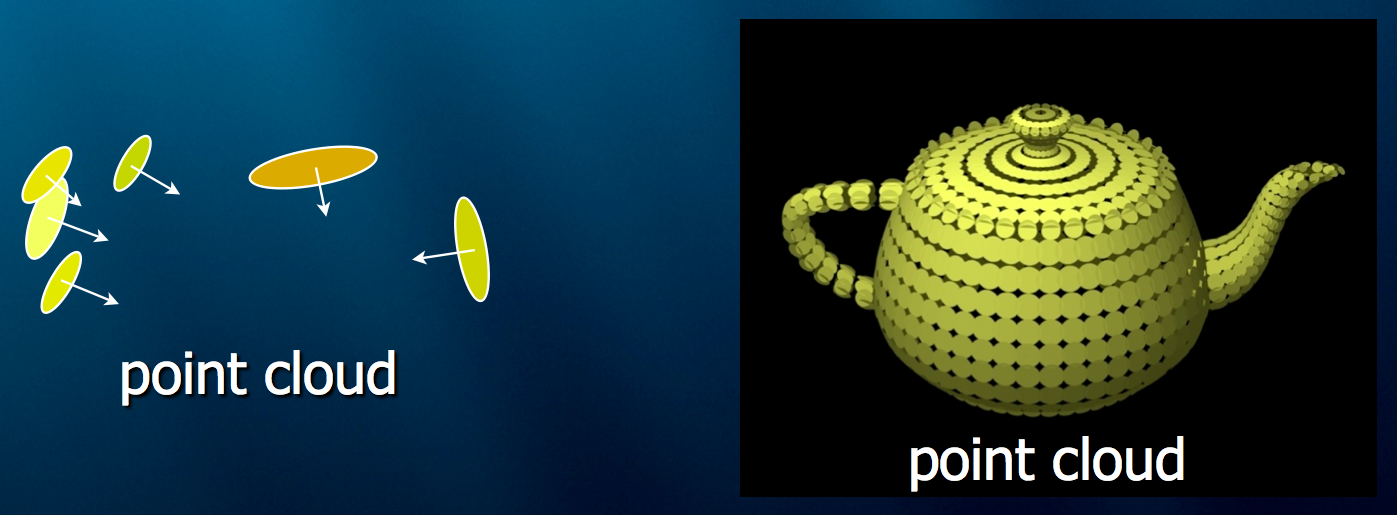
\includegraphics[width=150mm]{../img/surfel_disks.png}}
    \caption[Surfel Disks]{Surfels as disks, from Per H. Christensen's slides on the subject \cite{bib:christensen_slides}.}
    \label{fig:disk_surfels}
\end{figure}

During the course of the standard ray-tracing algorithm, the PBCB technique is used to compute the indirect illumination component required to shade an intersection point. For one point, a 5-faced cube-map is constructed such that each face is composed of an 8-by-8 pixel texture. This approximates the hemisphere used in the Monte Carlo gather technique (see Figure \ref{fig:monte_carlo}). The surfels are then convolved onto the cube-map using a proprietary algorithm \cite{bib:christensen2008}. What we do know about the algorithm is that, for very close surfels, rays are traced through the pixel to perform accurate shading, for average distance, the surfels are directly rasterized, and for distant surfels, a node from the surfel octree is used as an average representation of all the surfels in that area (see Figure \ref{fig:3_level_surfel}). Figure \ref{fig:surfel_raster} illustrates the result.

\begin{figure}
    \centering
    \subfloat{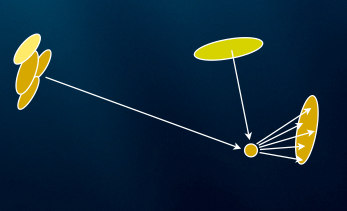
\includegraphics[width=100mm]{../img/surfel_raster_3_levels.png}}
    \caption[3 levels of surfel fidelity]{Close surfels are ray-traced, at average distance they are rasterized directly, and at long distance they are averaged \cite{bib:christensen_slides}.}
    \label{fig:3_level_surfel}
\end{figure}


With the surfel cloud rasterized onto the cube-map, each pixel represents the incoming radiance from its direction. The center of the pixel can be interpreted as if it were a sample point on the unit-hemisphere and the pixel's color can be weighted using the $n \cdot l$ factor to compute the incoming radiance value from that angle. These incoming radiance values are scaled by the surface color (see Section \ref{sec:phong_model}) and averaged to compute the final indirect illumination contribution to the shading computation for an intersection point.

